\section{Vorwort}

\section{Grundlagen von Mesh Netzen}

\begin{figure} [htbp]
	\centering
		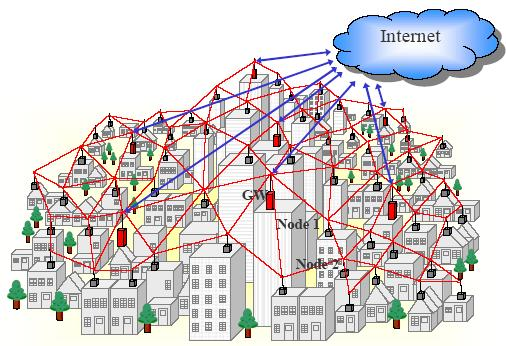
\includegraphics[width=0.50\textwidth]{WMN}
	\caption{Mesh Netz}
	\label{fig:WMN}
\end{figure}


\begin{verbatim}
  Position := Wurzel;  
  for i in 1..m do
    if (Position = Kante) then	
      if Zeichen auf dem Pfad im Baum = s'(i) then   
\end{verbatim}